% ==========================================
% BAB I PENDAHULUAN
% ==========================================
\chapter{PENDAHULUAN}
\label{chap:pendahuluan}

% --- 1.1 Latar Belakang ---
\section{Latar Belakang}

Kemajuan \textit{Large Language Models (LLM)} seperti \textit{GPT}, \textit{LLaMA}, dan \textit{PaLM} telah menghadirkan perubahan fundamental dalam berbagai aspek kehidupan modern. Model-model ini mampu menghasilkan teks yang koheren, mengikuti instruksi, serta membantu proses analisis informasi secara cepat dan efisien. Hal tersebut membuat LLM semakin banyak digunakan dalam layanan publik, pendidikan, kesehatan, bisnis, hingga penyediaan informasi sehari-hari \parencite{math2024hallucination}.

Namun, di balik kemajuan tersebut, terdapat tantangan serius berupa fenomena \textit{hallucination}. \textit{Hallucination} terjadi ketika model menghasilkan informasi yang tampak meyakinkan tetapi sebenarnya tidak benar, tidak berdasar, atau sepenuhnya fiktif \parencite{lettucedetect2024}. Risiko tersebut bukan sekadar isu teknis karena dampaknya telah terlihat nyata dalam berbagai kasus yang merugikan masyarakat.

Sebagai contoh nyata, pada tahun 2023 seorang pengacara di New York mengajukan rujukan kasus hukum fiktif hasil \textit{ChatGPT} hingga dikenai sanksi pengadilan \parencite{schwartz2023chatgptlawcase}, dan pada tahun 2024 \textit{chatbot} resmi maskapai Air Canada memberikan informasi keliru sehingga maskapai tersebut dinyatakan bertanggung jawab secara hukum \parencite{aircanada2024refundcase}. Khusus pada domain kesehatan yang menuntut akurasi tinggi, studi MedPaLM menunjukkan bahwa LLM masih kerap menghasilkan rekomendasi medis yang tidak akurat dan berpotensi membahayakan pasien jika digunakan tanpa verifikasi profesional \parencite{singhal2023medpalm}. Contoh-contoh ini menegaskan bahwa \textit{hallucination} merupakan isu kritis yang memengaruhi kepercayaan dan keamanan teknologi berbasis LLM, sehingga diperlukan upaya sistematis untuk memitigasinya, khususnya pada pendekatan \textit{Retrieval-Augmented Generation} (RAG) yang menggabungkan kemampuan generatif dengan sumber informasi eksternal.

Secara teoretis, RAG dapat mengurangi \textit{hallucination} karena model menjawab berdasarkan dokumen yang dapat diverifikasi. Namun dalam praktiknya, RAG tetap dapat menghasilkan informasi keliru apabila dokumen yang diperoleh tidak relevan, ambigu, atau tidak sesuai dengan maksud pertanyaan. Dengan demikian, kualitas jawaban tidak hanya bergantung pada kemampuan model generatif, tetapi juga pada proses pencarian dan pemilihan konteks yang tepat.

Tinjauan terbaru oleh Zhang (2025) berjudul \textit{“Hallucination Mitigation for Retrieval-Augmented Large Language Models: A Review”} memetakan berbagai penyebab \textit{hallucination} dalam RAG serta merangkum strategi mitigasinya \parencite{math2024hallucination}. Meskipun memberikan gambaran yang komprehensif, tinjauan tersebut menunjukkan bahwa solusi yang ada saat ini masih cenderung berdiri sendiri dan belum digabungkan dalam satu sistem terpadu. Sebagai contoh, Ma dkk.\ (2023) berfokus pada \textit{query rewriting} untuk memperbaiki formulasi kueri tanpa menyertakan \textit{reranking} konteks \parencite{ma2023queryrewriting}, sementara pendekatan seperti \textit{Chain-of-Verification} hanya menekankan mitigasi pada tahap \textit{generation} melalui verifikasi mandiri terhadap jawaban yang dihasilkan \parencite{dhuliawala2024cove}. Di sisi lain, sebagian penelitian lain berfokus pada \textit{context reranking} untuk menyaring dokumen hasil \textit{retrieval} \parencite{craft2023richresponses}. Pemisahan fokus ini menunjukkan adanya peluang untuk menggabungkan beberapa teknik mitigasi yang saling melengkapi dalam satu alur sistem yang utuh.

Salah satu penyebab spesifik halusinasi pada sistem RAG di domain biomedis adalah \textit{vocabulary mismatch}, yaitu ketidaksesuaian istilah antara pertanyaan pengguna dan teks dokumen yang menjadi korpus. Fenomena ini sangat sering dijumpai pada literatur biomedis karena dokumen ilmiah, khususnya abstrak paper di PubMed, banyak menggunakan akronim atau singkatan untuk istilah panjang. Sebagai contoh, istilah \textit{Hyperbaric Oxygen} ditulis dengan singkatan HBO, \textit{Coronary Heart Disease} ditulis dengan singkatan CHD, dan \textit{Body Mass Index} ditulis dengan singkatan BMI. Akibatnya, ketika pengguna mengajukan pertanyaan dengan istilah panjang yang lengkap, sistem \textit{retrieval} sering gagal menemukan dokumen relevan yang sebenarnya tersedia karena dokumen tersebut hanya mengandung versi akronimnya. Kegagalan \textit{retrieval} ini kemudian diteruskan ke tahap \textit{generation} dan menjadi salah satu pemicu halusinasi. Tahap praproses dokumen, khususnya ekspansi akronim biomedis, menjadi salah satu pendekatan yang berpotensi untuk mengatasi keterbatasan ini.

Selain praproses dokumen, sejumlah teknik mitigasi telah dikembangkan untuk memperbaiki kualitas \textit{retrieval} maupun \textit{generation} pada sistem RAG. Dua teknik yang banyak dibahas adalah \textit{query rewriting} (QR) dan \textit{context reranking} (CR) \parencite{math2024hallucination}. \textit{Query rewriting} bekerja pada tahap sebelum \textit{retrieval} dengan menulis ulang atau memperluas pertanyaan pengguna agar lebih sesuai dengan istilah yang digunakan pada korpus, sehingga peluang menemukan dokumen yang relevan menjadi lebih besar. Sementara itu, \textit{context reranking} bekerja setelah \textit{retrieval} dengan mengurutkan ulang dokumen kandidat berdasarkan tingkat relevansinya terhadap pertanyaan, sehingga dokumen yang paling relevan ditempatkan pada urutan teratas sebelum diteruskan ke tahap \textit{generation}.

Meskipun teknik-teknik tersebut telah terbukti efektif secara individual, sebagian besar studi hanya menerapkan satu jenis mitigasi pada satu tahap tertentu. Akibatnya, belum terdapat implementasi yang mengintegrasikan beberapa teknik mitigasi dalam satu alur menyeluruh untuk menekan halusinasi secara lebih efektif, khususnya pada domain biomedis yang memiliki karakteristik unik seperti \textit{vocabulary mismatch} akibat penggunaan akronim. Kesenjangan ini menjadi penting untuk diatasi, terutama pada bidang yang membutuhkan tingkat kebenaran informasi yang tinggi, seperti layanan publik, kesehatan, dan penegakan hukum.

% --- 1.2 Rumusan Masalah ---
\section{Rumusan Masalah}

Berdasarkan latar belakang tersebut, tugas akhir ini berfokus untuk menjawab beberapa pertanyaan utama sebagai berikut:
\begin{enumerate}
    \item Bagaimana arsitektur sistem RAG-LLM untuk mitigasi halusinasi pada sistem tanya jawab biomedis dirancang dan diimplementasikan dengan mengintegrasikan ekspansi akronim, \textit{query rewriting}, dan \textit{context reranking}?
    \item Bagaimana kontribusi komparatif setiap teknik mitigasi terhadap penurunan halusinasi dan peningkatan kualitas jawaban sistem?
\end{enumerate}

% --- 1.3 Tujuan ---
\section{Tujuan}

Tujuan dari tugas akhir ini adalah sebagai berikut:
\begin{enumerate}
    \item Merancang dan mengimplementasikan arsitektur sistem RAG-LLM untuk mitigasi halusinasi pada sistem tanya jawab biomedis dengan mengintegrasikan ekspansi akronim, \textit{query rewriting}, dan \textit{context reranking} sehingga dapat memproses pertanyaan biomedis secara otomatis.
    \item Menyusun analisis komparatif kontribusi setiap teknik mitigasi terhadap penurunan halusinasi dan peningkatan kualitas jawaban sistem.
\end{enumerate}

\section{Batasan Masalah}

Penelitian ini memiliki batasan ruang lingkup yang spesifik untuk
menjamin fokus kajian dan kelayakan penyelesaian dalam jangka waktu
pengerjaan tugas akhir. Berikut adalah batasan masalah yang ditetapkan:

\begin{enumerate}
    \item Penelitian ini menggunakan \textit{dataset}
          PubMedQA subset \textit{pqa\_labeled} yang berisi 1.000 paper
          biomedis berlabel \textit{expert} dari basis data PubMed.
          \textit{Dataset} pada domain lain di luar biomedis tidak
          termasuk dalam cakupan penelitian. Dari 1.000 paper
          tersebut, 500 pertanyaan pertama dipilih sebagai himpunan uji
          evaluasi. Jumlah korpus dan pertanyaan evaluasi ini dipilih
          untuk menjaga keseimbangan antara representativitas eksperimen
          dan keterbatasan sumber daya komputasi serta biaya pemanggilan
          API LLM.

    \item Halusinasi yang dianalisis dibatasi
          pada dua kategori yang paling relevan dengan proses
          \textit{retrieval} dan \textit{generation}, yaitu halusinasi
          intrinsik (keluaran yang bertentangan dengan konteks yang
          diberikan) dan halusinasi faktual (keluaran yang mengandung
          informasi keliru meskipun tampak meyakinkan). Jenis halusinasi
          lain seperti \textit{reasoning}, \textit{linguistic}, dan
          \textit{bias-related hallucination} tidak termasuk dalam
          cakupan.

    \item Teknik mitigasi yang diimplementasikan
          dibatasi pada tiga pendekatan utama, yaitu ekspansi akronim
          biomedis menggunakan algoritma Schwartz-Hearst sebagai tahap
          praproses dokumen, \textit{query rewriting} berbasis
          \textit{Large Language Model} untuk perluasan kueri, dan
          \textit{context reranking} untuk menata ulang dokumen kandidat
          berdasarkan relevansi. Metode mitigasi lain seperti
          \textit{prompt engineering} lanjutan, \textit{knowledge
          editing}, atau \textit{model fine-tuning} tidak dibahas dalam
          penelitian ini.

    \item Model bahasa yang digunakan terbatas
          pada empat model, yaitu Llama 3.2, Llama 3.3, GPT-4.1, dan
          Claude 4.5. Seluruh model diakses melalui API berbayar dengan
          pemilihan \textit{tier} atau varian yang paling ekonomis pada
          masing-masing model untuk menyesuaikan dengan keterbatasan
          biaya pada pengerjaan tugas akhir. Model bahasa lain di luar
          keempat model tersebut tidak termasuk dalam cakupan
          implementasi.

    \item Seluruh data,
          \textit{prompt}, dan proses \textit{retrieval} dilakukan
          menggunakan bahasa Inggris. Penelitian tidak mencakup analisis
          pada bahasa lain di luar bahasa Inggris.

    \item Evaluasi kinerja sistem dilakukan
          menggunakan kombinasi tiga jenis metrik, yaitu (a) metrik
          kualitas \textit{retrieval} seperti \textit{nDCG@k},
          \textit{MAP@k}, dan \textit{Recall@k}; (b) metrik akurasi
          klasifikasi label (\textit{accuracy} terhadap \textit{ground
          truth} \textit{yes/no/maybe}); dan (c) metrik \textit{Retrieval
          Augmented Generation Assessment} (RAGAS) yang meliputi
          \textit{faithfulness}, \textit{context recall}, \textit{answer
          relevancy}, dan \textit{context precision}.
\end{enumerate}.

% ==========================================
% 1.5 Metodologi Tugas Akhir (versi umum)
% ==========================================
\section{Metodologi Tugas Akhir}

Tugas akhir ini menggunakan pendekatan metodologi \textit{Cross-Industry Standard Process for Data Mining} atau disingkat \textbf{CRISP-DM}. Metodologi ini merupakan kerangka kerja industri yang banyak digunakan dalam proyek berbasis \textit{data mining} dan \textit{machine learning} karena bersifat fleksibel, iteratif, serta berorientasi pada kebutuhan bisnis dan teknis \parencite{crispdm_datasciencepm}.

CRISP-DM menyediakan tahapan sistematis untuk memahami permasalahan, menyiapkan data, membangun model, hingga mengevaluasi serta mengimplementasikannya. Metodologi ini terdiri atas enam fase utama, yaitu: \textit{business understanding}, \textit{data understanding}, \textit{data preparation}, \textit{modeling}, \textit{evaluation}, serta \textit{deployment}.

Visualisasi tahapan metodologi \textit{CRISP-DM} dapat dilihat pada Gambar~\ref{gambar:crispdm}.

\begin{figure}[H]
  \centering
  \captionsetup{justification=centering}
  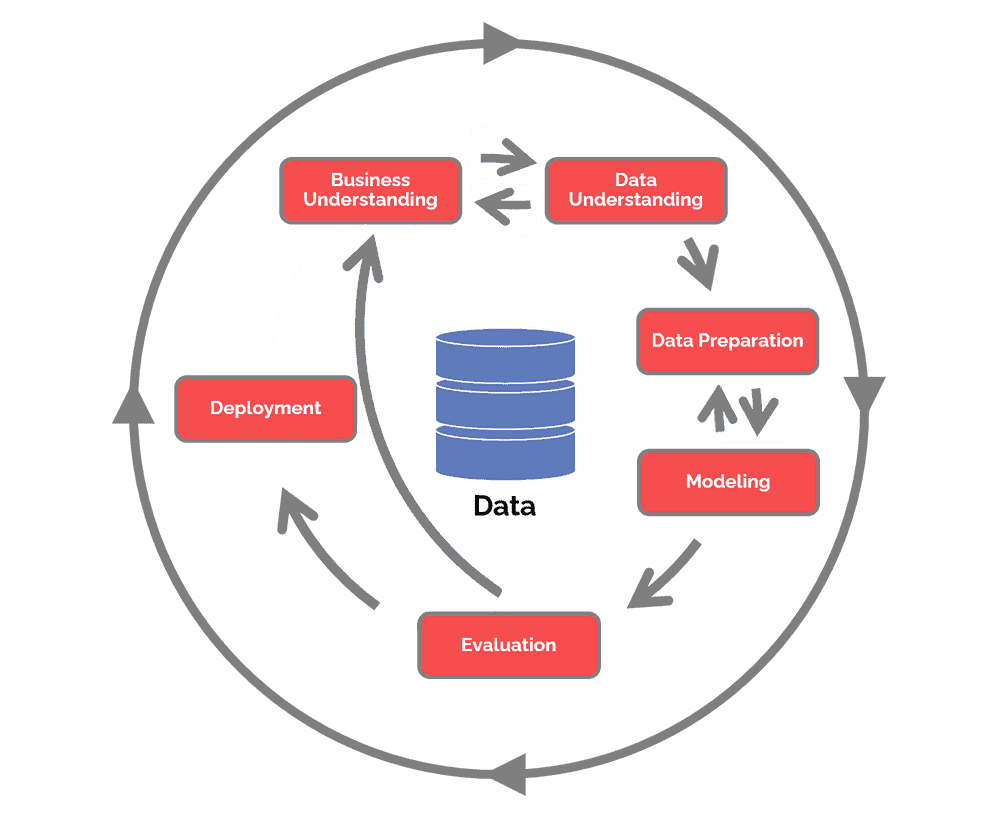
\includegraphics[width=0.85\textwidth]{image/crispdm.png}
  \caption[Tahapan Metodologi CRISP-DM]{Tahapan Metodologi CRISP-DM \parencite{crispdm_datasciencepm}}
  \label{gambar:crispdm}
\end{figure}

\subsection{\textit{Business Understanding}}
Tahap pertama bertujuan memahami kebutuhan dan tujuan sistem dari sudut pandang pengguna atau masalah operasional. Kegiatan dilakukan untuk menentukan ruang lingkup, sasaran, serta kriteria keberhasilan model yang akan dibangun. Pemahaman konteks pada fase ini menjadi fondasi dalam pemilihan strategi analisis dan pendekatan pemodelan.

\subsection{\textit{Data Understanding}}
Tahap ini berfokus pada eksplorasi data awal, termasuk identifikasi sumber data, penilaian kualitas, serta analisis karakteristik yang relevan dengan permasalahan. Tujuannya adalah memperoleh wawasan mengenai struktur, konten, serta permasalahan yang mungkin muncul pada tahap pemrosesan.

\subsection{\textit{Data Preparation}}
Tahap ini mencakup pembersihan data, seleksi variabel, penggabungan data, transformasi format, serta penanganan \textit{missing values}. Hasil akhir tahap ini adalah dataset terstruktur dengan kualitas memadai untuk digunakan pada proses pemodelan.

\subsection{\textit{Modeling}}
Pada tahap ini ditentukan teknik pemodelan, pemilihan algoritma, serta konfigurasi parameter (\textit{hyperparameter}) yang sesuai. Data yang telah dipersiapkan kemudian digunakan untuk membangun model, termasuk pengujian alternatif parameter untuk mendapatkan kinerja yang optimal.

\subsection{\textit{Evaluation}}
Tahap ini mengevaluasi kinerja model berdasarkan metrik evaluasi kuantitatif. Selain itu, dilakukan pula pengecekan kesesuaian model dengan tujuan tugas akhir. Apabila model belum memenuhi kriteria keberhasilan, diperlukan iterasi kembali pada tahap pemahaman data atau pemodelan.

\subsection{\textit{Deployment}}
Tahap terakhir adalah penerapan model ke dalam lingkungan operasional atau simulasi implementasi. Pada tahap ini dilakukan pemantauan performa, dokumentasi, serta pengelolaan perubahan data dan model agar solusi tetap andal dalam jangka panjang. Pada tugas akhir ini, tahap \textit{deployment} dibatasi pada simulasi \textit{pipeline} sistem RAG dan tidak mencakup penerapan berskala produksi (\textit{production-scale deployment}).

Metodologi CRISP-DM menyediakan kerangka terstruktur yang menyeimbangkan kebutuhan teknis dan praktis sehingga tugas akhir berbasis data dapat dijalankan secara sistematis, transparan, dan dapat direproduksi dengan baik.
